\chapter{Subsistema de adquisición}

El subsistema de adquisición es el encargado de recibir la señal analógica
procedente del subsistema para la interacción con el medio físico,
muestrearla y proporcionar a las capas superiores una versión digital de la
misma. Es un subsistema exclusivo, y al mismo tiempo distintivo de los
sistemas digitales de medida. En la \cref{fig:subacqui} se muestra una
ventana parcial del sistema de medida digital centrada en las unidades
funcionales que conforman el subsistema de adquisición.

\begin{figure}
	\begin{center}
		\includegraphics{gis-pfc-ch2-01.mps}
	\end{center}
	\caption[Subsistema de adquisición] {Elementos funcionales que
	incluye el subsistema de adquisición.}
	\label{fig:subacqui}
\end{figure}

El subsistema de adquisición del sistema digital de medida propuesto para
el proyecto comprende un único bloque, un bloque de adquisición en el que
se ubica una tarjeta de adquisición. La tarjeta \kpci{} es el fundamento en
el que se basa, no sólo el subsistema de adquisición, si no el sistema
digital de medida al completo. Sus capacidades y muchas de sus limitaciones
las hereda el sistema, y constituyen los principios de diseño del resto de
subsistemas. El subsistema para la interacción con el medio debe proveer al
subsistema de adquisición con una señal que se ajuste a las
especificaciones de la tarjeta, además el circuito acondicionador de
recepción debe adaptar la impedancia de entrada mostrada por el
dispositivo. Por su parte, el subsistema de control y presentación debe ser
capaz de gestionar el funcionamiento de este instrumento y administrar los
valores de señal que proporciona. Además, la \kpci{}, disponer de ella, es
una de las razones principales por las que se ha optado por desarrollar un
sistema de adquisición propio, de propósito, sin tener en cuenta las
principales razones, como es obvio, uno de los objetivos del proyecto,
adquirir conocimientos prácticos en el campo del tratamiento digital de
señales y, por supuesto, contar con un sistema diseñado a medida. Por todas
estas razones, resulta comprensible realizar un estudio previo acerca de
las propiedades y el comportamiento de un instrumento de tan singular
importancia para este proyecto.

Esta memoria dedica un capítulo completo a exponer las características de
la tarjeta \kpci{}. Una breve relación de las características técnicas del
hardware da paso a la descripción funcional, en la que se explica cual es
el comportamiento interno de la tarjeta, como se implementan las distintas
funciones que ofrece. Para terminar el capítulo se reproducen los consejos
que el fabricante proporciona en el manual de usuario con la premisa de que
los usuarios consigan el máximo rendimiento de la tarjeta (punto
\ref{sec:throughput} en la página \pageref{sec:throughput}) y se muestra la
caja de conexiones elaborada expresamente para este proyecto.


\section{Características técnicas del hardware}\label{sec:technical}

La tarjeta \kpci{} puede emplearse para la adquisición y conversión de
señales analógicas en señales digitales, para sintetizar señales analógicas
a partir de señales digitales previamente generadas o almacenadas, o
---gracias a sus 32 puertos digitales de propósito general--- trabajar con
señales digitales.

El subsistema de adquisición dentro del sistema de medida digital requiere
únicamente de la función de adquisición analógica de la tarjeta. Por ello,
de entre todas las características del dispositivo, se ha creído
conveniente resumir a continuación aquellas que tienen relación directa con
dicha función. Para obtener información detallada sobre la relación que
estos atributos guardan con el proceso de adquisición de señales analógicas
en la tarjeta \kpci{}, véase la \vref{sec:funcdesc}.

\begin{itemize}
	\item El módulo de adquisición analógica dispone de 16 puertos
		físicos.
	\item La impedancia de entrada equivalente de cada puerto es
		aproximadamente igual a una capacidad de 200 pF en serie
		con una resistencia de valor inferior, pero aproximadamente
		igual, a 1 k$\Omega$.
	\item En condiciones óptimas, es posible conseguir un rendimiento
		máximo de 100 \kms{} (cien mil operaciones de conversión
		por segundo). Este valor está sujeto a un error relativo
		del $0.02\%$.
	\item La resolución del conversor analógico digital es de 16 bits
		por muestra. El rango de amplitudes en el que opera depende
		de como esté configurado el modo de adquisición. Puede ir
		de 0 V a 10 V si el modo de adquisición es unipolar, o de
		-10 V a 10 V si es bipolar.
	\item La cola de muestreo tiene capacidad para hasta 256 canales
		distintos. Cada uno de los cuales puede configurarse
		independientemente en términos de ganancia, frecuencia de
		muestreo, modo de adquisición o modo de terminación.
	\item La ganancia, responsable en parte de la resolución con la que
		se cuantifica las muestras, puede tomar cada ciclo de reloj
		uno de entre 16 valores posibles (véase el
		\vref{tab:acqmodes}).
\end{itemize}


\section{Descripción funcional}\label{sec:funcdesc}

Es necesario programar el comportamiento de la tarjeta de adquisición antes
de ponerla en funcionamiento. Desde la cola de muestreo se controlan los
principales aspectos del proceso de adquisición, como por ejemplo, en que
instantes se encuentra activo.

La cola de muestreo, como su propio nombre indica, es una estructura de
datos ordenada. Se encuentra almacenada en una memoria \sig{ram} de 256
entradas que forma parte del hardware de la tarjeta. En el \cref{tab:queue}
puede verse una representación de un ejemplo de la cola de muestreo.

\begin{table}
	\centering
	\begin{threeparttable}
	\begin{tabular}{lccccccccc}
		\toprule
		Posición en la cola & 1 & 2 & 3 & 4 %
		& \multicolumn{2}{c}{$\cdots$} & 254 & 255 & 256 \\
		\midrule
		Número de canal & 15 & 15 & 02 & 02 %
		& \multicolumn{2}{c}{$\cdots$} & 17 & 13 & 01 \\
		Número de puerto & 07 & 07 & 11 & 11 %
		& \multicolumn{2}{c}{$\cdots$} & 07 & 09 & 01 \\
		Ganancia & 1 & 1 & 40 & 40 %
		& \multicolumn{2}{c}{$\cdots$} & 200 & 8 & 80 \\
		Modo de adquisición\tnote{a} & $\pm$ & $\pm$ & $+$ & $+$ %
		& \multicolumn{2}{c}{$\cdots$} & $\pm$ & $+$ & $\pm$ \\
		Modo de terminación\tnote{b} & \sig{d} & \sig{d} %
		& \sig{m} & \sig{m} & \multicolumn{2}{c}{$\cdots$} %
		& \sig{d} & \sig{m} & \sig{m}\\
		\bottomrule
	\end{tabular}
	\begin{TableNotes}
		\tnotetext{a}{Configuración bipolar ($\pm$), configuración
		unipolar ($+$).}
		\tnotetext{b}{Canal diferencial (\sig{d}), canal
		monoterminal (\sig{m}).}
	\end{TableNotes}
	\end{threeparttable}
	\caption[Ejemplo de cola de muestreo]{Ejemplo de cola de muestreo.}
	\label{tab:queue}
\end{table}

Cada entrada en la memoria \sig{ram} se identifica con una posición en la
cola. Las posiciones en la cola pueden encontrarse vacías o estar ocupadas
por un canal. Varias posiciones en la cola, consecutivas o no, pueden estar
ocupadas por un mismo canal. Por tanto, la cola puede estar ocupada, como
máximo, por 256 canales independientes.

Las posiciones ocupadas contienen información correspondiente al canal y a
los atributos asociados a este. Un canal es una entidad lógica que
relaciona un puerto físico con un búffer de información y una serie de
atributos. Durante el proceso de adquisición un puntero recorre las
distintas posiciones de la cola, una a una y en orden. El canal activo,
aquel que ocupa la posición a la que apunta el puntero en cada ciclo de
reloj, determina tres cosas:

\begin{itemize}
	\item De qué puerto debe proceder la señal analógica\footnote{Por
		convenio se ha elegido hablar de una sola señal que entra
		al amplificador. Si se ha hecho esta elección, es porque si
		bien al amplificador pueden entrar una o dos señales
		simultáneamente, esto no supone otra diferencia para el
		proceso que la expuesta en el \vref{subsubsec:termmodes}.
		Es por ello, y para mantener la claridad, que se ha omitido
		esta posibilidad.} que llega al amplificador de
		instrumentación interno de la tarjeta.
	\item En qué búffer debe almacenarse el valor resultante de
		muestrear y cuantificar esta señal.
	\item Por último, los atributos asociados al canal: ganancia, modo
		de adquisición y modo de terminación; indican,
		respectivamente: cual debe ser la ganancia del amplificador
		de instrumentación, cual debe ser el rango de trabajo del
		conversor analógico digital, y que se debe conectar a los
		terminales de entrada del amplificador de instrumentación.
		Se da más información al respecto en apartados
		subsiguientes.% la polaridad de las muestras y el número de
		% terminales de entrada, uno o dos dependiendo de si la
		% adquisición es diferencial o no, durante el ciclo actual.
\end{itemize}

Para concluir el apartado cabe remarcar lo siguiente. Es posible inferir
dos cosas de esta mecánica de funcionamiento basada en la cola. Una de
ellas es que el proceso de adquisición afecta a una sola señal cada vez. Y
la segunda, que la frecuencia de muestreo ligada a un canal depende de dos
factores, de la velocidad de la señal de reloj, y de la cantidad de veces
que un canal aparece repetido en la cola.


\subsection{Métodos de entrada}

La \kpci{} permite dos modos de adquisición y dos modos de terminación.
Aprender a diferenciar cuando es oportuno seleccionar entre cada uno de
ellos beneficiará la calidad de la señal digital resultante.


\subsubsection{Modos de adquisición}

Una señal es bipolar cuando toma valores positivos y negativos. Por el
contrario, se distingue a las señales unipolares porque todos sus valores
mantienen la misma polaridad, ya sea ésta positiva o negativa. Para cada
canal, debe configurarse el modo de adquisición como bipolar o
unipolar\footnote{La tarjeta \kpci{} sólo admite señales unipolares de
polaridad positiva.} atendiendo a la señal de interés.

Si se sabe a ciencia cierta que la señal de entrada es unipolar debe
emplearse el modo de adquisición unipolar. De ese modo, se duplica la
resolución del conversor analógico digital.

\begin{sidewaystable}
	\centering
	\begin{tabular}{>{\raggedleft}p{1.2cm}d{5.2}d{3.1}+d{3.1}}
		\toprule
		& \multicolumn{2}{c}{Bipolar} %
		& \multicolumn{2}{c}{Unipolar} \\
		\cmidrule(r){2-3}\cmidrule(l){4-5}
		\multicolumn{1}{c}{Ganancia}
		& \multicolumn{1}{c}{Rango ($\pm\text{V}$)} %
		& \multicolumn{1}{c}{Precisión ($\mu\text{V}$)} %
		& \multicolumn{1}{c}{Rango (V)} %
		& \multicolumn{1}{c}{Precisión ($\mu\text{V}$)} \\
		\midrule
		1 & 10,0 & 305 & 0/$10,0$ & 153 \\
		2 & 5,0 & 153 & 0/$5,0$ & 76 \\
		4 & 2,5 & 76 & 0/$2,5$ & 38 \\
		8 & 1,25 & 38 & 0/$1,25$ & 19 \\
		10 & 1,0 & 31 & 0/$1,0$ & 15 \\
		\\
		& \multicolumn{2}{c}{Bipolar} %
		& \multicolumn{2}{c}{Unipolar} \\
		\cmidrule(r){2-3}\cmidrule(l){4-5}
		\multicolumn{1}{c}{Ganancia}
		& \multicolumn{1}{c}{Rango ($\pm\text{mV}$)} %
		& \multicolumn{1}{c}{Precisión ($\mu\text{V}$)} %
		& \multicolumn{1}{c}{Rango (mV)} %
		& \multicolumn{1}{c}{Precisión ($\mu\text{V}$)} \\
		\midrule
		20 & 500 & 15 & 0/500 & 7,6 \\
		40 & 250 & 7,6 & 0/250 & 3,8 \\
		80 & 125 & 3,8 & 0/125 & 1,9 \\
		100 & 100 & 3,1 & 0/100 & 1,5 \\
		200 & 50 & 1,5 & 0/50 & 0,8 \\
		400 & 25 & 0,8 & 0/25 & 0,4 \\
		800 & 12,5 & 0,4 & 0/$12,5$ & 0,2 \\
		\bottomrule
	\end{tabular}
	\caption[Ganancia del amplificador y precisión del
	conversor]{Relación entre ganancia, rango de trabajo y resolución
	según el modo de adquisición.}
	\label{tab:acqmodes}
\end{sidewaystable}


\subsubsection{Modos de terminación}\label{subsubsec:termmodes}

Internamente, la tarjeta \kpci{} emplea un amplificador de instrumentación
diferencial. En principio este hecho implicaría que a cada canal se
asociasen dos puertos físicos, uno por cada uno de los dos terminales de
entrada del amplificador. No obstante, es posible configurar la tarjeta
para que uno de los terminales del amplificador se conecte a masa. En ese
caso, el terminal restante se conecta a un puerto físico. La
\vref{fig:termmodes} muestra un ejemplo de esta configuración.

\begin{figure}
	\begin{center}
		\includegraphics{gis-pfc-ch2-02.mps}
	\end{center}
	\caption[Ejemplo de configuración de terminación]{Figura que
	muestra el modo de terminación sencillo. La entrada superior del
	amplificador de instrumentación se conecta al puerto 9 y la entrada
	inferior se conecta a masa.}
	\label{fig:termmodes}
\end{figure}

Para habilitar semejante configuración, cabría pensar que es suficiente con
modificar el atributo que controla el modo de terminación del canal
correspondiente. Al contrario de lo que pudiera parecer, el modo de
terminación es una propiedad que no es atribuible al canal, si no que se
atribuye a un par de puertos\footnote{Aunque según las especificaciones del
fabricante es posible configurar cada par de puertos para que opere según
un modo de terminación independiente del resto, el entorno de desarrollo
utilizado durante el proyecto sólo admite un modo de terminación para el
conjunto total de puertos (v. el \vref{chap:control}).}. En concreto, el
modo de terminación afecta a los pares de puertos compuestos por un primero
de entre los puertos 0 y 7, y un segundo cuyo número de puerto es igual al
del primero más 8. De ahí que todos los canales relacionados con el mismo
par de puertos deban estar configurados con el mismo modo de terminación,
una configuración distinta no está permitida.

Los dos modos de terminación posibles se conocen como: diferencial, si es
que la señal que entra en cada terminal del amplificador procede de cada
uno de los puertos del par; sencillo, en caso de que uno de los terminales
de entrada del amplificador se conecte a la referencia de tensión. En este
documento se llama canal diferencial a los canales cuyo modo de terminación
sea diferencial, y canal con un sólo terminal o monoterminal a aquellos
para los que el modo de terminación es sencillo.

Las ventajas que presenta el uso de uno u otro tipo de canales son
comprensibles. Emplear canales con un sólo terminal permite aplicar el
proceso de adquisición sobre un mayor número de señales simultáneamente.
Por el contrario, utilizar canales diferenciales redunda en una mayor
inmunidad frente al ruido. Además, los amplificadores diferenciales
eliminan de forma inherente la componente en continua.


\section{Rendimiento}\label{sec:throughput}

En el ámbito de este documento se entiende como rendimiento de la tarjeta
de adquisición la cantidad máxima de operaciones de conversión que el
dispositivo puede realizar por unidad de tiempo. Para que una de estas
operaciones contribuya a la medida de rendimiento debe superar un requisito
de precisión.

El rendimiento óptimo de la tarjeta \kpci{} especificado por el fabricante
es de cien mil operaciones por segundo (100 \kms{}). No obstante se
advierte, para obtener este nivel de rendimiento es necesario alimentar la
tarjeta con una fuente de tensión ideal. Además, es importante que exista
adaptación de impedancias entre el circuito de alimentación y el puerto por
el que se quiere introducir la señal. Aún en estas condiciones el valor
proporcionado por la casa Keithley está sujeto a un error relativo máximo
del $0.02\%$, el cual supone un error absoluto máximo de dos mil
operaciones por segundo (2 \kms{}).

En los \sig{endus}, existe una relación directa entre la resolución, la
capacidad de distinguir entre dos defectos próximos, y la frecuencia de
oscilación de la señal ultrasónica. Cuanto mayor sea la frecuencia de las
ondas acústicas mejor la resolución. Los transductores utilizados en el
ensayo se comportan como filtros además de como transductores, ya que por
un lado sólo dejan pasar determinadas componentes de frecuencia y por otro
transforman variaciones de la tensión eléctrica en variaciones de presión o
viceversa. Imponen un límite físico a la frecuencia de oscilación de la
señal ultrasónica y, por tanto, en la resolución. Para trabajar con señales
acústicas de alta frecuencia son necesarios transductores adecuados que
presenten un gran ancho de banda y sean capaces de transmitir las altas
frecuencias. El receptor transforma el pulso acústico en un pulso eléctrico
filtrado, después esta señal se acondiciona y deja el subsistema para la
interacción con el medio físico para pasar al subsistema de adquisición. En
el subsistema de adquisición el pulso eléctrico se muestrea y es ahí donde
entra en juego el rendimiento de la \kpci{}. El teorema de Nyquist estipula
una frecuencia de muestreo mínima para la cual no se produce una pérdida de
información al muestrear una señal periódica y limitada en banda. La
frecuencia de Nyquist es igual al doble de la frecuencia de oscilación
máxima de la señal que se preve muestrear. Si una señal se muestrea a una
tasa inferior se da una pérdida de información y no es posible recuperar la
señal original. En otras palabras, para una frecuencia de muestreo fija,
sólo las señales que oscilan a frecuencias por debajo de la mitad de la
frecuencia de muestreo son correctamente muestreadas. De lo que se deduce
que, cuanto mayor sea el rendimiento del bloque de adquisición, mayor la
frecuencia de las señales que pueden muestrearse sin pérdidas, lo que
implica que no existe impedimento para emplear un receptor de mayor
frecuencia, y asimismo es posible alcanzar una mejor resolución en los
ensayos. Si se emplean transductores de alta frecuencia, y el receptor
genera una señal de frecuencia superior a la mitad del rendimiento del
dispositivo de adquisición, el beneficio de trabajar con señales de alta
frecuencia no es real. Este es el principal motivo que fomenta el interés
por extraer el mayor rendimiento de la tarjeta \kpci{}. Para lograrlo es
necesario conocer por un lado que factores limitan el rendimiento de la
tarjeta y, por otro, como debe configurarse el dispositivo para que la
influencia de esos factores sea mínima.


\subsection[El amplificador de instrumentación] {Amplificador de
instrumentación y pérdida del rendimiento}

El amplificador de instrumentación interno de la \kpci{} es de ganancia
variable. Es posible configurar una ganancia distinta para cada canal. El
propósito del amplificador es permitir al usuario modificar la amplitud de
la señal que entra al conversor. La intención que se persigue es conseguir
que la conversión se enfoque en los detalles de la señal que sean de mayor
interés y se pierda la mínima información posible. Todo ello aún trabajando
simultáneamente con múltiples señales cuyo rango de amplitudes es con
frecuencia muy diferente.

La desventaja que presenta esta configuración ---multiplexor, amplificador
de instrumentación, conversor--- es una pérdida de rendimiento que se
produce en situaciones determinadas a causa de la intervención del
amplificador en la operación de adquisición.

Cada ciclo de reloj cambia el canal activo y debe cambiar, si es oportuno,
la señal que accede al amplificador. Este proceso no es inmediato. Tras
conmutar el multiplexor que precede al amplificador, se da paso al puerto
conveniente. No obstante, la señal que recibe el amplificador presenta,
hasta transcurrido un determinado periodo de tiempo, una componente
residual de la señal que se amplificó en el anterior ciclo de reloj.
Transcurrido dicho periodo de tiempo la señal que entra al amplificador se
ve libre de esa componente residual y se corresponde únicamente con la
señal que entrega el multiplexor, se dice que se ha fijado la señal.

Y es así como el amplificador es causa de pérdida de rendimiento, por medio
de las componentes residuales. Si la conversión se realiza antes de fijar
la señal, el conversor toma un valor de la señal corrompido por la
componente residual de la señal precedente. Por tanto, la muestra
resultante queda igualmente corrompida incluso hasta el punto de perder su
validez. Las operaciones de conversión que tengan como resultado muestras
inválidas sólo contribuyen a falsear la medida de rendimiento, haciendo que
parezca mayor de lo que en realidad es.

El fabricante da a entender que existe una solución de diseño que resuelve
en parte el problema planteado por las componentes residuales. Esta
solución consiste en alargar de forma deliberada la duración del ciclo de
reloj, de esa forma se proporciona tiempo suficiente para fijar la señal.
Sin embargo, esta solución presenta dos inconvenientes: no solventa el
problema en la totalidad de los casos y es, asimismo, una forma de perder
rendimiento. Lo cual conduce inevitablemente a una solución de compromiso,
alargar el ciclo de reloj lo suficiente para que en la mayoría de los casos
el efecto de las componentes residuales sobre la precisión de la conversión
no invalide las muestras resultantes y se produzca, por tanto, una caída
del rendimiento, sin que la duración del nuevo ciclo contribuya por sí
misma a una pérdida notable de éste.


\subsection{Factores que limitan el rendimiento}

Como se ha visto, la inclusión del amplificador en el diseño de la tarjeta
es causa directa o indirecta de una pérdida de rendimiento. La magnitud de
esa caída en el rendimiento depende de la configuración de la cola de
muestreo y de la amplitud de la señal una vez llega ésta al dispositivo de
adquisición.

\subsubsection{Pequeña señal}

Las señales cuya tensión absoluta se encuentra por debajo de los 100 mV al
llegar a la \kpci{} sufren en mayor medida las consecuencias del empleo de
un amplificador en la operación de conversión. En primer lugar la señal
tarda más en fijarse de modo que el rendimiento se reduce a la mitad en las
mejores condiciones, de 100 \kms{} pasa a 50 \kms{}. Esto es debido a que,
al ser la amplitud de la señal y la del ruido comparables, especialmente
después de que éste se vea reforzado por el efecto de las componentes
residuales, se genera una mayor incertidumbre.

Por otro lado las señales que requieren que el amplificador opere con alta
ganancia son las más perjudicadas por los problemas que causa el
amplificador en configuraciones multiganancia, tal y como se explica a
continuación.


\subsubsection{Configuraciones multiganancia}

Por lo general, el rendimiento se ve afectado de forma más pronunciada por
el efecto de las componentes residuales en configuraciones multiganancia en
las que se encadenan secuencias de canales con ganancia diferente. Una
configuración multiganancia de la cola de muestreo implica que en
diferentes ciclos de reloj el amplificador actúa con ganancias distintas.
Eso con frecuencia significa que el rango en el que se encuentra
comprendida la amplitud de las señales que están entrando al dispositivo de
adquisición es diferente de una señal a otra. Cuando así ocurre puede
sucederse en ocasiones que en ciclos de reloj consecutivos entren al
amplificador dos señales de amplitud diferente, siendo la amplitud de la
señal que ocupa el primer ciclo mucho mayor que la de la otra señal en el
tiempo en el que ambas permanecen a la entrada del dispositivo. Por otro
lado, parece lógico considerar que la componente residual asociada a una
señal cuya amplitud sea predominantemente mayor que la de otra señal es de
mayor amplitud inicial y mayor duración temporal que la asociada a la
segunda señal. Por tanto si ocurre como se ha dicho y se tiene en cuenta la
base probable que se ha propuesto, cuando la segunda de las señales se
convierte en la señal activa la amplitud de la componente residual asociada
a la primera de ellas puede ser suficiente, incluso, para enmascararla.

No sólo eso, la amplitud de la señal que llega más tarde al amplificador
puede ser, en términos absolutos, la mayor parte del tiempo, menor que la
de la otra señal, al ser así lo más probable es que se amplifique empleando
un mayor factor de ganancia. De ser así, la amplitud de la componente
residual a la que se enfrenta esta señal puede provocar en el peor de los
casos que el conversor sature y la pérdida de precisión sea mucho mayor.
Sea cual sea el caso, es posible observar entonces, que en configuraciones
multiganancia las muestras resultantes se obtienen de una conversión menos
precisa, en especial si se trabaja con señales de pequeña amplitud ---tal y
como se especificó en el punto anterior--- o si las ganancias configuradas
en la cola de muestreo difieren mucho unas de otras. Aplicando la relación
entre la validez de las muestras y el rendimiento de la que se habló
anteriormente, la consecuencia de emplear configuraciones multiganancia es
una mayor pérdida de rendimiento.


\subsubsection{Configuraciones monoganancia}

En configuraciones monoganancia el uso del amplificador supone una causa
indirecta de la caída de rendimiento. El diseño del dispositivo de
adquisición está pensado primordialmente para su uso en configuraciones
multiganancia, de lo contrario la inclusión de un amplificador de ganancia
variable en el esquemático de la tarjeta sería incomprensible. Por la misma
razón, Keithley adopta una solución de diseño como la expuesta en el
anterior apartado, para tratar de obtener un rendimiento óptimo en
configuraciones multiganancia. Sin embargo, el efecto de las componentes
residuales en configuraciones monoganancia es mínimo y la consecuente
pérdida de rendimiento también lo es. Por tanto, una solución que consiste
en alargar el ciclo de reloj resulta, en configuraciones monoganancia,
innecesaria y perjudicial para el rendimiento.


\subsection{Configuración óptima de la cola de muestreo}

Las acciones que el fabricante adopta para tratar de que el usuario obtenga
el mayor rendimiento posible del dispositivo no se limitan a aplicar una
solución de compromiso en el diseño de la duración del ciclo de reloj. En
el manual de usuario se hacen una serie de recomendaciones de uso
orientadas a conseguir este fin.

Se proponen varias soluciones, de las cuales la solución trivial pasa por
preamplificar todas las señales que vayan a ser objeto del proceso de
adquisición efectuado por la tarjeta consiguiendo que su amplitud varíe en
un mismo rango. Si se hace así, es suficiente con emplear una configuración
monoganancia para minimizar los efectos de las componentes residuales en el
rendimiento. Además al preamplificar las señales, éstas presentan una mejor
relación señal a ruido, es decir, son menos vulnerables al ruido. Aunque
buena, esta solución no deja de ser trivial puesto que el amplificador de
instrumentación de la tarjeta pierde toda funcionalidad y pasa a ser un
estorbo en el proceso de adquisición.

La solución de carácter práctico propuesta por Keithley radica configurar
la cola de muestreo de forma minuciosa, persiguiendo optimizar el
rendimiento. Como se ha visto, en determinadas ocasiones una configuración
inapropiada de la cola de muestreo puede inducir que la pérdida de
productividad que provoca la inclusión del amplificador en el circuito de
adquisición sea todavía mayor. Para evitar que esto ocurra y sacar el
máximo partido del dispositivo se dan en el manual dos condiciones que de
cumplirse garantizan que la cola se encuentre configurada de forma óptima
en términos de rendimiento.


\subsubsection{Agrupaciones de canales}

La primera consiste en agrupar canales con distinta ganancia en posiciones
consecutivas de la cola, aún si al hacerlo se pierde el orden de muestreo
definido en una primera instancia por el usuario. Si como se presupuso en
el apartado anterior, comúnmente dos señales que requieren ser amplificadas
con el mismo factor de ganancia varían en el mismo rango de amplitudes, en
estas secuencias monoganancia las consecuencias de las componentes
residuales en la precisión de la conversión son mínimas.


\subsubsection{Posciones consecutivas}

A pesar de emplear una configuración como la anterior, la aparición de
saltos de ganancia en la cola de muestreo es todavía probable. Por ejemplo,
en la transición entre dos secuencias monoganancia como las descritas
arriba. El salto es aún más problemático si la transición se realiza para
dar paso a una secuencia de ganancia mayor. El primer canal de esta
secuencia sufre en mayor proporción los efectos de las componentes
residuales y el rendimiento asociado al canal se ve reducido
dramáticamente. Para minimizar el impacto que en determinados canales como
éste tienen los problemas causados por el amplificador, es posible
modificar la configuración de la cola para que dichos canales ocupen varias
posiciones consecutivas. Esta segunda condición persigue dar más tiempo
para que se fije la señal cuando los mencionados canales están activos.
Para ello se necesitan posiciones vacías en la cola, posiciones que es
posible obtener desalojando canales previamente configurados.


\section{Comunicación con el periférico}

Para la interacción con dispositivos externos, la \kpci{} dispone de dos
conectores formato mini-\sig{d} de 36 terminales que cumplen con el
estándar \sig{ieee} 1284 de protocolos de comunicación en paralelo. Si se
observa la tarjeta como el rectángulo que forma desde un punto de vista
geométrico y observándola de frente, los conectores quedan ubicados en un
lado de la tarjeta contiguo a aquel en el que se sitúa la conexión
\sig{pci}. Todo ello de forma que tras el montaje del periférico en la
placa base los conectores quedan expuestos en la parte posterior de la
carcasa en la que providencialmente debe encontrarse instalada dicha placa,
tal y como es habitual en este tipo de dispositivos.

En las \cref{fig:portanalog,fig:portdigital} se etiqueta cada terminal
según su ubicación relativa con respecto al conector y al resto de
terminales en el mismo, para cada conector, mostrando la distribución
definida por el fabricante. Los \cref{tab:analog,tab:digital} describen el
propósito de cada terminal y se especifica que tipo de señal debe circular
por los mismos.

\begin{figure}
	\begin{center}
		\subfloat[Conector etiquetado como \guillemotleft
		analog\guillemotright][Conector etiquetado como
		\guillemotleft analog\guillemotright.]{ %
			\label{fig:portanalog} %
			\includegraphics{gis-pfc-ch2-03.mps}}
			\vspace*{.1\textheight}
		\subfloat[Conector etiquetado como \guillemotleft
		digital\guillemotright][Conector etiquetado como
		\guillemotleft digital\guillemotright.]{ %
			\label{fig:portdigital} %
			\includegraphics{gis-pfc-ch2-04.mps}}
	\end{center}
	\caption[Conectores traseros de la tarjeta de adquisición]
	{Conectores traseros de la tarjeta de adquisición.}
	\label{fig:ports}
\end{figure}

\newlength\tablewidth
\setlength\tablewidth{.5\linewidth}

\begin{table}
	\centering
	\begin{tabular}%
		{>{\raggedleft}p{1cm} >{\scshape}c >{\arraybackslash}l}
		\toprule
		\multicolumn{1}{c}{Terminal} & {\upshape Puerto asignado} %
		& \multicolumn{1}{c}{Descripción} \\
		\midrule
		1 & ip5 & \multirow{16}{\tablewidth}{Bits digitales de
		entrada multifunción. Pueden ser configurados por el
		usuario para que ejerzan la función de:\miniit{\item Base
		temporal para el contador/temporizador y/o entrada a
		\emph{gate} \\\item Reloj externo para conversiones A/D o
		D/A \\\item Disparador digital externo \\\item Entrada
		digital en el modo \emph{target-mode}}} \\
		2 & ip3 & \\
		3 & ip1 & \\
		\\\\\\\\\\\\\\\\\\\\\\\\
		\midrule
		4 & op5 & \multirow{16}{\tablewidth}{Bits digitales de
		salida multifunción. Pueden ser configurados por el usuario
		para que ejerzan la función de:\miniit{\item Salidas del
		contador/temporizador\\\item Salida del disparador\\\item
		Salida de control para accesorios\\\item Salida del reloj
		interno\\\item Salida digital en el modo
		\emph{target-mode}}} \\
		5 & op3 & \\
		6 & op1 & \\
		\\\\\\\\\\\\\\\\\\\\\\\\
		\bottomrule
	\end{tabular}
	\caption[Mapa de terminales del conector \emph{analog}]{Relación
	entre los puertos y terminales que presenta el conector trasero de
	la \kpci{} etiquetado como \emph{analog}.}
	\label{tab:analog}
\end{table}

\begin{table}\ContinuedFloat
	\centering
	\begin{tabular}%
		{>{\raggedleft}p{1cm} >{\scshape}c >{\arraybackslash}l}
		\toprule
		\multicolumn{1}{c}{Terminal} & {\upshape Puerto asignado}
		& \multicolumn{1}{c}{Descripción} \\
		\midrule
		7 & dgnd & Tierra digital \\
		\midrule
		8 & ch07 lo/ch15 & \multirow{5}{\tablewidth}{Entradas
		analógicas, cuya función depende del modo de terminación
		configurado: puerto asociado a un canal monoterminal o
		puerto bajo de un canal diferencial} \\
		9 & ch06 lo/ch14 & \\
		10 & ch05 lo/ch13 & \\
		\multicolumn{1}{c}{$\vdots$} & $\vdots$ & \\
		15 & ch00 lo/ch08 & \\
		\midrule
		16 & {\upshape Sin conexión} & \\
		\midrule
		\multicolumn{1}{l}{17, 18} & agnd & Tierra analógica \\
		\midrule
		19 & ip4 & \multirow{16}{\tablewidth}{Bits digitales de
		entrada multifunción. Pueden ser configurados por el
		usuario para que ejerzan la función de:\miniit{\item Base
		temporal para el contador/temporizador y/o entrada a
		\emph{gate} \\\item Reloj externo para conversiones A/D o
		D/A \\\item Disparador digital externo \\\item Entrada
		digital en el modo \emph{target-mode}}} \\
		20 & ip2 & \\
		21 & ip0 & \\
		\\\\\\\\\\\\\\\\\\\\\\\\
		\bottomrule
	\end{tabular}
	\caption[]{Continuación del \vref{tab:analog}.}
\end{table}

\begin{table}\ContinuedFloat
	\centering
	\begin{tabular}%
		{>{\raggedleft}p{1cm} >{\scshape}c >{\arraybackslash}l}
		\toprule
		\multicolumn{1}{c}{Terminal} & {\upshape Puerto asignado} %
		& \multicolumn{1}{c}{Descripción} \\
		\midrule
		22 & op4 & \multirow{16}{\tablewidth}{Bits digitales de
		salida multifunción. Pueden ser configurados por el usuario
		para que ejerzan la función de:\miniit{\item Salidas del
		contador/temporizador\\\item Salida del disparador\\\item
		Salida de control para accesorios\\\item Salida del reloj
		interno\\\item Salida digital en el modo
		\emph{target-mode}}} \\
		22 & op2 & \\
		21 & op0 & \\
		\\\\\\\\\\\\\\\\\\\\\\\\
		\midrule
		25 & {\upshape +5 V} & \multirow{3}{\tablewidth}{Referencia
		de tensión de 5 voltios de corriente continua extraídos del
		bus \sig{pci} del ordenador} \\
		\\\\
		\midrule
		26 & ch07 hi & \multirow{4}{\tablewidth}{Entradas
		analógicas restantes, en el modo de terminación diferencial
		representan el puerto alto de un canal diferencial} \\
		27 & ch06 hi & \\
		28 & ch05 hi & \\
		\multicolumn{1}{c}{$\vdots$} & $\vdots$ & \\
		33 & ch00 hi & \\
		\bottomrule
	\end{tabular}
	\caption[]{Continuación del \vref{tab:analog}.}
\end{table}

\begin{table}\ContinuedFloat
	\centering
	\begin{tabular}%
		{>{\raggedleft}p{1cm} >{\scshape}c >{\arraybackslash}l}
		\toprule
		\multicolumn{1}{c}{Terminal} & {\upshape Puerto asignado} & \multicolumn{1}{c}{Descripción} \\
		\midrule
		34 & {\upshape +10 V} & \multirow{9}{\tablewidth}{Entrada
		diseñada para proporcionar al dispositivo una referencia
		externa de precisión de 10 voltios mediante una fuente de
		alta impedancia de salida (La impedancia de entrada de este
		puerto es equivalente a una resistencia de 1 k$\Omega$ en
		serie con la impedancia de entrada de la fuente)} \\
		\\\\\\\\\\\\\\\\
		\midrule
		35 & dac1 & \multirow{2}{\tablewidth}{Salida número 1 del
		conversor digital a analógico de la \kpci{}} \\
		\\
		\midrule
		36 & dac0 & \multirow{2}{\tablewidth}{Salida número 0 del
		conversor digital a analógico de la \kpci{}} \\
		\\
		\bottomrule
	\end{tabular}
	\caption[]{Continuación del \vref{tab:analog}.}
\end{table}

\begin{table}
	\centering
	\begin{tabular}%
		{>{\raggedleft}p{1cm} >{\scshape}c >{\arraybackslash}l}
		\toprule
		\multicolumn{1}{c}{Terminal} & {\upshape Puerto asignado} & \multicolumn{1}{c}{Descripción} \\
		\midrule
		1 & {\upshape Bit 0} & \multirow{8}{\tablewidth}{Canal 0 de
		bits de entrada/salida de propósito general (En la \kpci{}
		los bits digitales se agrupan de en ocho en ocho en
		canales. Los canales de este tipo puede configurarse para
		que los bits que lo integran se comporten como todo salidas
		o todo entradas)} \\
		2 & {\upshape Bit 1} & \\
		3 & {\upshape Bit 2} & \\
		\multicolumn{1}{c}{$\vdots$} & $\vdots$ & \\
		8 & {\upshape Bit 7} & \\
		\\\\\\
		\midrule
		9 & {\upshape Bit 8} & \multirow{2}{\tablewidth}{Canal 1 de
		bits de entrada/salida de propósito general} \\
		10 & {\upshape Bit 9} & \\
		11 & {\upshape Bit 10} & \\
		\multicolumn{1}{c}{$\vdots$} & $\vdots$ & \\
		16 & {\upshape Bit 15} & \\
		\midrule
		\multicolumn{1}{l}{17, 18} & dgnd & Tierras digitales \\
		\midrule
		19 & {\upshape Bit 16} & \multirow{2}{\tablewidth}{Canal 2
		de bits de entrada/salida de propósito general} \\
		20 & {\upshape Bit 17} & \\
		21 & {\upshape Bit 18} & \\
		\multicolumn{1}{c}{$\vdots$} & $\vdots$ & \\
		26 & {\upshape Bit 23} & \\
		\midrule
		27 & {\upshape Bit 24} & \multirow{2}{\tablewidth}{Canal 3
		de bits de entrada/salida de propósito general} \\
		28 & {\upshape Bit 25} & \\
		29 & {\upshape Bit 26} & \\
		\multicolumn{1}{c}{$\vdots$} & $\vdots$ & \\
		34 & {\upshape Bit 31} & \\
		\midrule
		\multicolumn{1}{l}{35, 36} & {\upshape +5 V} %
		& +5 V\sig{dc} desde el bus del ordenador \\
		\bottomrule
	\end{tabular}
	\caption[Mapa de terminales del conector \emph{digital}]{Relación
	entre los puertos y terminales que presenta el conector trasero de
	la \kpci{} etiquetado como \emph{digital}.}
	\label{tab:digital}
\end{table}


\subsection{Desarrollo de una nueva interfaz}\label{subsec:conbox}

Por razones prácticas, la interfaz original de la \kpci{} basada en dos
conectores mini-\sig{d} no se acomoda a las necesidades que se prevé
surgirán durante el desarrollo de las pruebas requeridas para la
finalización de este proyecto de fin de carrera. En consecuencia, con el
propósito de agilizar en la medida de lo posible la realización de estos
ensayos, se decide ampliar la interfaz existente.

Para ello se parte de dos extremos de cable terminados en un conector tipo
macho y desprovistos de cubierta, de cada uno de los cuales surgen 36 hilos
de cobre recubiertos de plástico flexible coloreado. El patrón de coloreado
de las cubiertas individuales es único y no se repite en ninguno de los 36
hilos de que se compone cada extremo de cable. A partir de ahí, se
identifica cada terminal de cada conector con el hilo de cobre
correspondiente, relacionando las etiquetas que el fabricante pone a los
terminales con el código de colores de la cubiertas individuales.

Una vez recopilada esta información, se planea la construcción de una caja
de conexiones. El diseño de la caja contempla que se equipe ésta con 72
conectores banana hembra soldados a los 72 hilos de cobre y que comunican
con los terminales de los conectores mini-\sig{d} en los que termina el
otro extremo de los cables. Además se planifica la inclusión de cuatro
conectores coaxiales con rosca con conexiones redundantes a las que se
presupone son las cuatro puertas cuyo uso será más frecuente, las
correspondientes al primer canal analógico diferencial y las tierras
analógicas; para así facilitar el uso continuado de las mismas. Por último
se decide etiquetar la caja de conexiones con marbetes que reproduzcan la
nomenclatura visible en las \vref{fig:portanalog,fig:portdigital}.

Puede observarse una representación de la caja de conexiones ya terminada
en la \vref{fig:conbox}.

\begin{figure}
	\begin{center}
		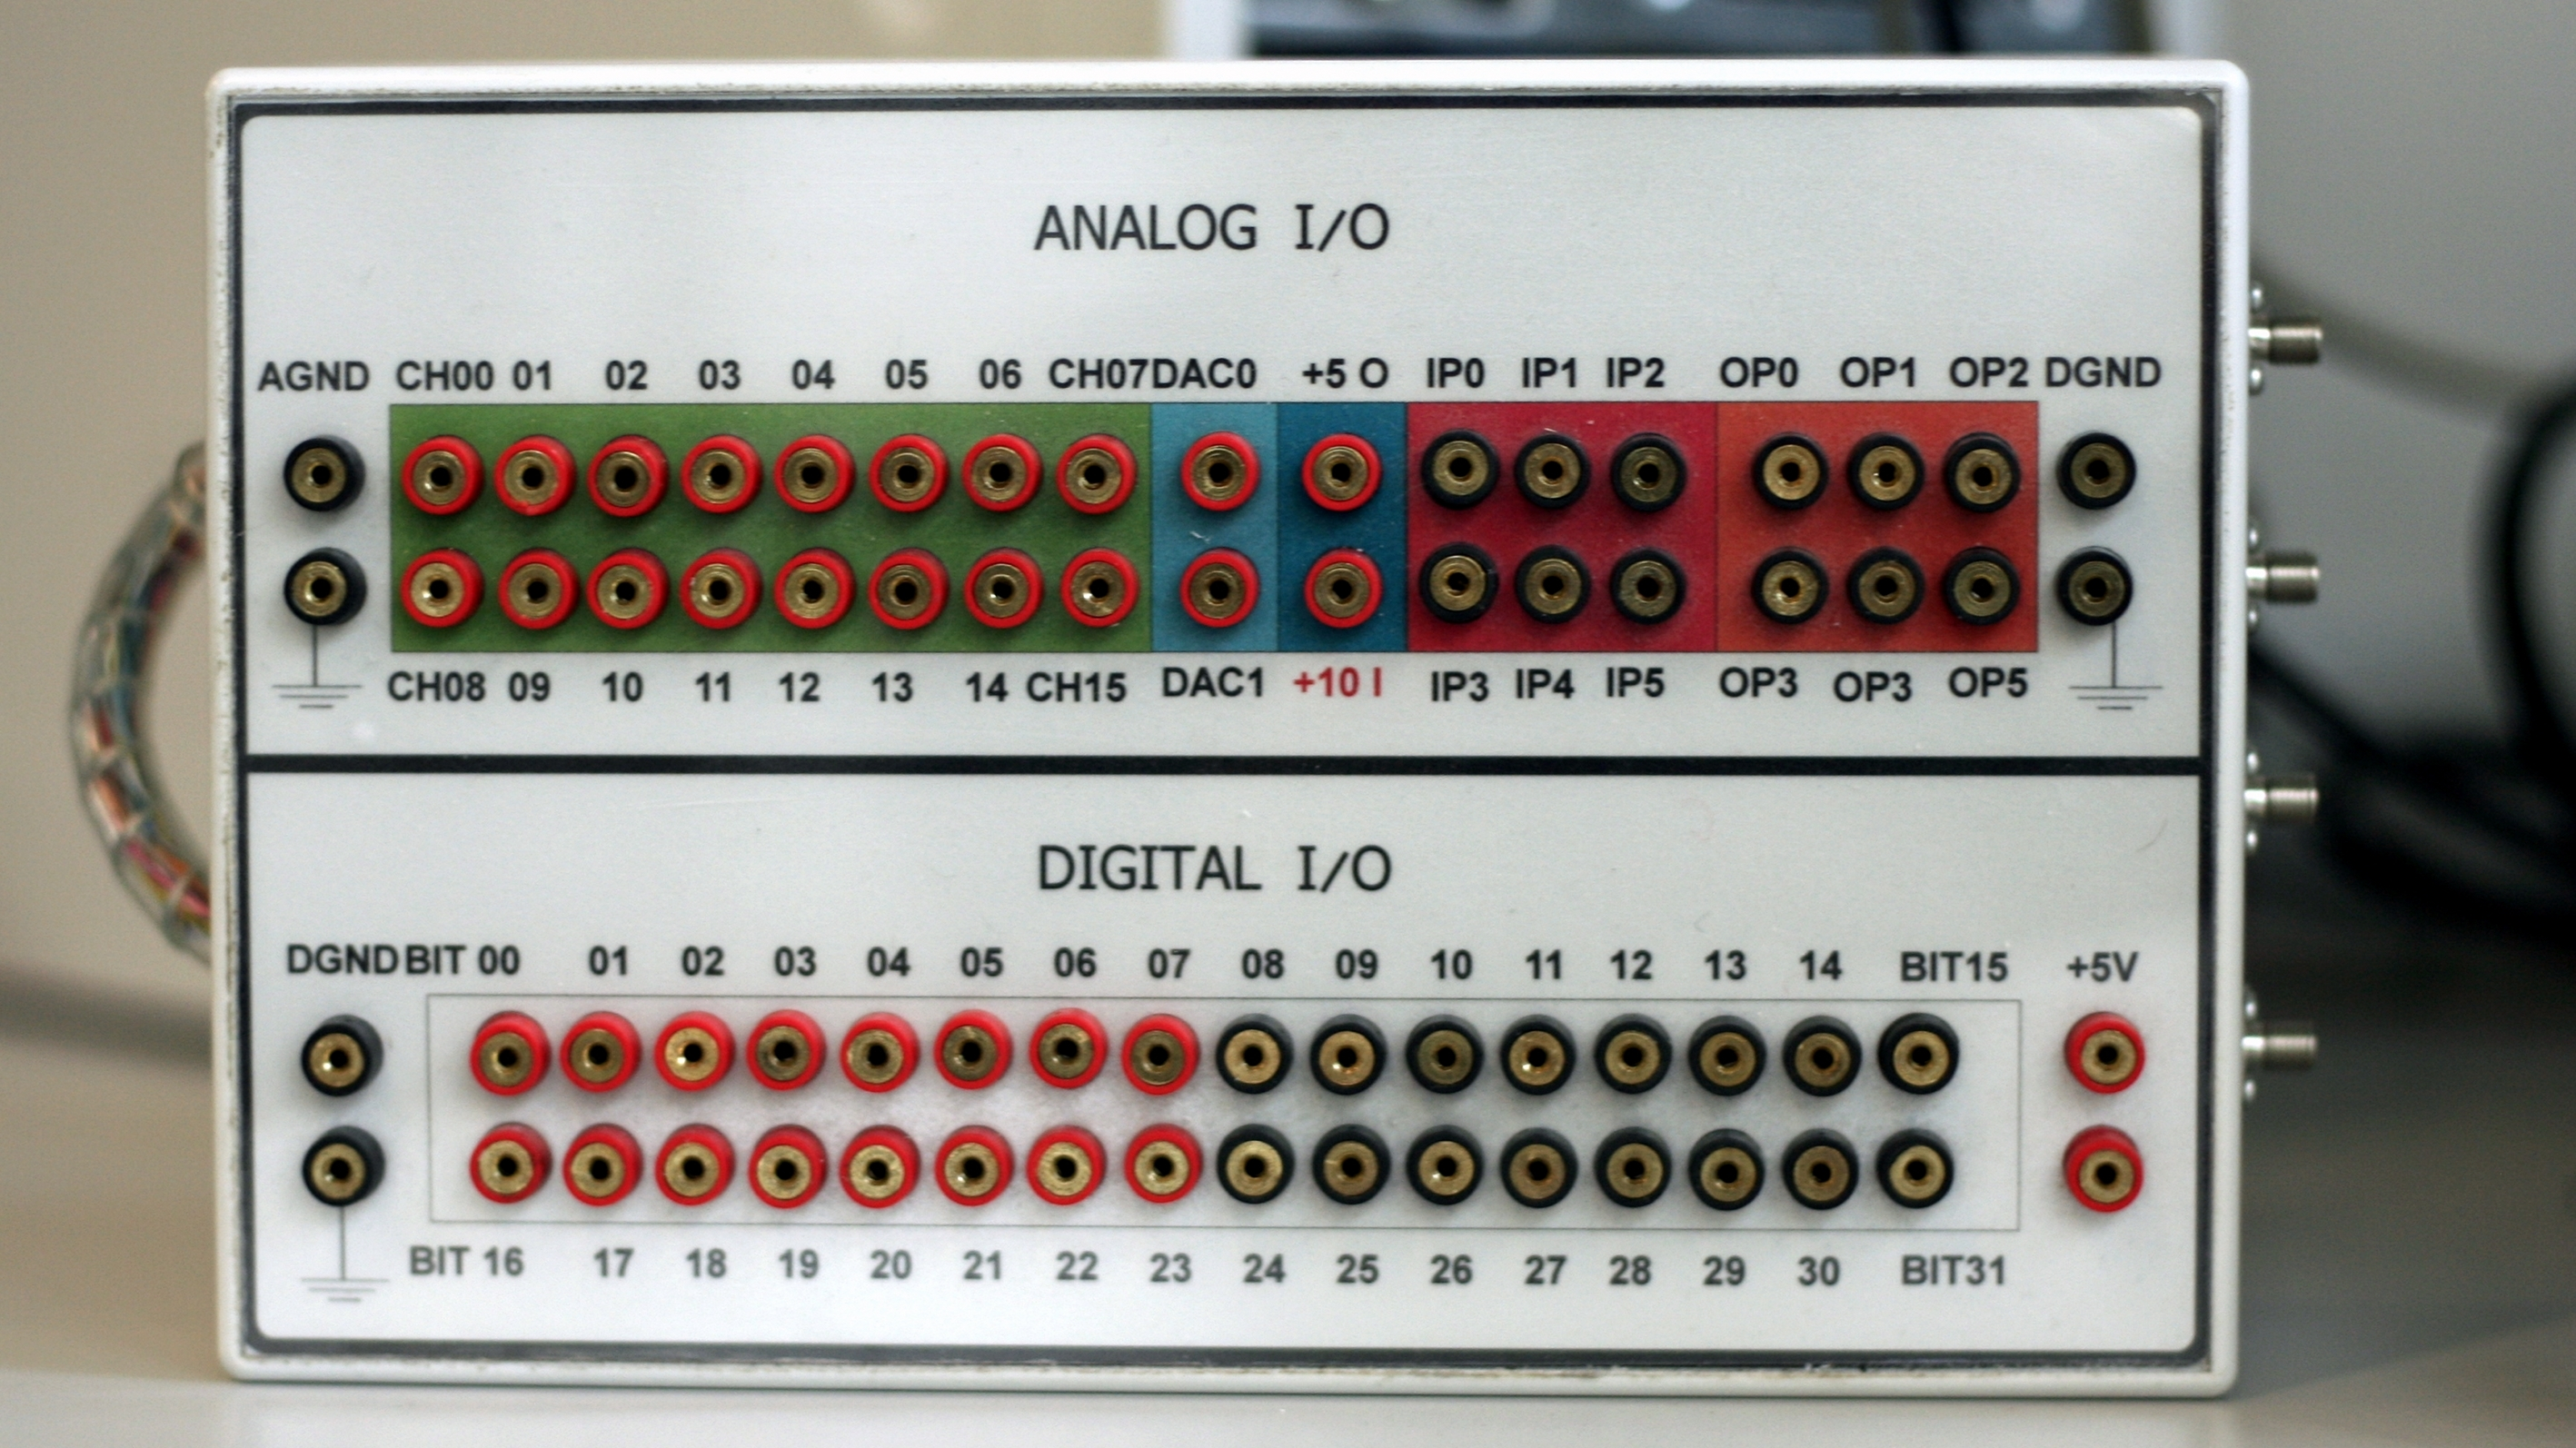
\includegraphics[scale=1, keepaspectratio=true]
		{gis-pfc-ch2-05.jpg}
	\end{center}
	\caption[Plano de la caja de conexiones ya terminada] {Plano de la
	caja de conexiones ya terminada.}
	\label{fig:conbox}
\end{figure}
